% chapters/methodology.tex  — Sections 5 and 6

\chapter{System Architecture and Implementation}{\label{ch:methodology}}

\section{High Level Architecture Overview}

At a high level, the system is composed of four primary layers:

\begin{itemize}
    \item \textbf{Frontend Layer (Client Side):} Provides the user interface for students, faculty, and
    administrators.
    \item \textbf{Backend Layer (Application Server):} Handles business logic, API processing, and
    authentication.
    \item \textbf{Database Layer:} Stores persistent data such as users, sessions, attendance, and
    feedback.
    \item \textbf{External Services Layer:} Includes integrations like email notifications and external
    platforms.
\end{itemize}

This layered structure ensures separation of concerns, improving maintainability and scalability.

% figs/arch_layers.tex — 4-layer architecture diagram
\begin{figure}[!ht]
\centering
\begin{tikzpicture}[font=\small, node distance=6pt]
  \node[layernode, text width=14cm, draw=softred, fill=redbg!60] (ext) at (7,7.8)
    {External Services Layer \quad {\footnotesize Email SMTP $\cdot$ Google OAuth $\cdot$ Google Classroom API}};
  \node[layernode, text width=14cm, draw=accentblue, fill=boxbg] (db) at (7,6.3)
    {Database Layer \quad {\footnotesize PostgreSQL via Supabase — Users $\cdot$ Sessions $\cdot$ Attendance $\cdot$ Feedback $\cdot$ Files}};
  \node[layernode, text width=14cm, draw=successgreen, fill=greenbg!60] (be) at (7,4.8)
    {Backend Layer \quad {\footnotesize Next.js API Routes — Auth $\cdot$ Scheduling $\cdot$ Attendance $\cdot$ Feedback $\cdot$ Reporting}};
  \node[layernode, text width=14cm, draw=warnorange, fill=orangebg!60] (fe) at (7,3.3)
    {Frontend Layer \quad {\footnotesize Next.js (React) — Admin Dashboard $\cdot$ Student Dashboard $\cdot$ Feedback UI}};

  \draw[myarrow] (fe.north) -- node[right,font=\scriptsize,color=midgray]{HTTP / REST} (be.south);
  \draw[myarrow] (be.north) -- node[right,font=\scriptsize,color=midgray]{SQL queries}  (db.south);
  \draw[myarrow] (be.east |- be.center) -- ++(0.6,0) |-
    node[near start,right,font=\scriptsize,color=midgray]{External calls} (ext.east);
\end{tikzpicture}
\caption{Four-layer high-level architecture of CIPD 360 ERP}
\label{fig:arch_layers}
\end{figure}


\section{Technology Stack}

The system is built using a modern web stack:

\begin{itemize}
    \item \textbf{Frontend:} Next.js for efficient rendering and interactivity
    \item \textbf{Backend:} API routes within Next.js for unified development
    \item \textbf{Database:} PostgreSQL (via Supabase) for reliable data storage
    \item \textbf{Authentication:} JWT based stateless authentication
    \item \textbf{Attendance System:} Wi Fi based device detection
    \item \textbf{Integrations:} OAuth support for external platforms
\end{itemize}

This stack balances performance, scalability, and development efficiency.

\section{Architectural Components and Responsibilities}

The system is divided into modular components:

\begin{itemize}
    \item \textbf{Authentication:} Manages user identity and access control
    \item \textbf{Scheduling:} Handles session planning and updates
    \item \textbf{Attendance:} Processes network data into attendance records
    \item \textbf{Feedback:} Manages feedback collection and analytics
    \item \textbf{Dashboard and Reporting:} Aggregates and visualizes system data
    \item \textbf{Coursework:} Handles materials, assignments, and grading
\end{itemize}

These components interact through well defined APIs, ensuring modularity.

\section{Data Flow and Processing Architecture}

The system follows a structured data flow:

\begin{enumerate}
    \item User actions on the frontend trigger API requests
    \item Backend processes requests using business logic
    \item Data is stored or retrieved from the database
    \item Responses are returned and rendered on the frontend
    \item Certain events trigger automated workflows
\end{enumerate}

Key automated workflows include:

\begin{itemize}
    \item \textbf{Attendance Processing:} Network data is analysed to generate attendance records
    \item \textbf{Session Lifecycle Handling:} Sessions transition through states (scheduled $\rightarrow$ ongoing
    $\rightarrow$ completed), triggering dependent processes
    \item \textbf{Feedback Activation:} Feedback forms are enabled automatically after session
    completion
\end{itemize}

This approach reduces manual effort and ensures consistency across modules.

% figs/wifi_pipeline.tex — WiFi detection pipeline diagram
\begin{figure}[!ht]
\centering
\begin{tikzpicture}[font=\small]
  \node[blknode=2.4cm] (router) at (0,    0) {Dedicated\\WiFi Router\\{\footnotesize 192.168.0.1}};
  \node[blknode=2.4cm] (script) at (3.2,  0) {Selenium\\Script\\{\footnotesize (24/7 PC)}};
  \node[blknode=2.4cm] (parse)  at (6.4,  0) {Parse MAC\\ + Signal\\Strength};
  \node[blknode=2.4cm] (filter) at (9.6,  0) {Threshold\\Filter\\{\footnotesize Signal $>2$}};
  \node[dbnode=2.4cm]  (map)    at (9.6, -2.4){Map to\\Registered\\Students};
  \node[dbnode=2.4cm]  (db)     at (6.4, -2.4){Update\\Attendance\\Records};

  \draw[myarrow] (router.east) -- (script.west);
  \draw[myarrow] (script.east) -- (parse.west);
  \draw[myarrow] (parse.east)  -- (filter.west);
  \draw[myarrow] (filter.south) -- (map.north);
  \draw[myarrow] (map.west)     -- (db.east);

  % labels
  \node[font=\scriptsize,color=midgray,above=3pt of router] {Step 1};
  \node[font=\scriptsize,color=midgray,above=3pt of script] {Step 2};
  \node[font=\scriptsize,color=midgray,above=3pt of parse]  {Step 3};
  \node[font=\scriptsize,color=midgray,above=3pt of filter] {Step 4};
  \node[font=\scriptsize,color=midgray,below=3pt of map]    {Step 5};
  \node[font=\scriptsize,color=midgray,below=3pt of db]     {Step 6};
\end{tikzpicture}
\caption{WiFi-based automated attendance detection pipeline}
\label{fig:wifi_pipeline}
\end{figure}


\section{Integration of Attendance Pipeline}

A key architectural feature of the system is the integration of the attendance pipeline with
the core application.

The process involves:

\begin{itemize}
    \item Collection of Wi Fi snapshot data from the network
    \item Mapping detected devices to registered users
    \item Processing detection data into attendance records
    \item Storing both raw and processed data for analysis
\end{itemize}

This pipeline operates alongside the main application and continuously feeds processed
attendance data into the database. The stored data is then utilized by dashboards, reporting
modules, and analytics systems.

By integrating this pipeline directly into the architecture, the system enables automated,
scalable, and data driven attendance tracking.

\section{Database Design Overview}

The system uses a relational database (PostgreSQL) to manage structured data across
modules.

Core entities include:

\begin{itemize}
    \item Users and roles
    \item Sessions and scheduling data
    \item Attendance records and device mappings
    \item Feedback forms and responses
    \item Assignments and submissions
\end{itemize}

Relationships ensure referential integrity and efficient querying. The schema is normalized to
reduce redundancy, with selective denormalization for faster analytics queries.

\section{API Design and Communication}

The system follows an API driven architecture for frontend backend interaction.

Key characteristics:

\begin{itemize}
    \item \textbf{Role Based Endpoints:} Separate APIs for admin, faculty, and students
    \item \textbf{Stateless Communication:} JWT based authentication
    \item \textbf{Structured Responses:} Consistent and enriched data formats
    \item \textbf{Error Handling:} Standardized responses for reliability
\end{itemize}

This design ensures extensibility and supports future integrations.

\section{Frontend Implementation}

The frontend is developed using Next.js with a focus on usability and performance.

Key aspects include:

\begin{itemize}
    \item Component based design for consistency
    \item Dynamic data fetching via APIs
    \item Responsive interfaces across devices
    \item State management for smooth interaction
\end{itemize}

\section{Integration of System Components}

The system ensures seamless interaction between modules:

\begin{itemize}
    \item Scheduling drives attendance and feedback workflows
    \item Attendance data feeds dashboards and reporting
    \item Feedback data contributes to analytics and evaluation
\end{itemize}

This integration enables cohesive system behaviour across all components.

% ─────────────────────────────────────────────────────────────────────────────
\chapter{Module wise Design}{\label{ch:modules}}
% ─────────────────────────────────────────────────────────────────────────────

\section{Authentication and User Management}

The Authentication and User Management module forms the foundational layer of the CIPD 360 ERP
system. It is responsible for establishing user identity, enforcing access control, and enabling secure
interaction across all system components. As all modules depend on user specific behavior, this
module acts as the entry point and control boundary for the system.

\subsection{Role Based Access Control}

The system is structured around two primary roles:

\begin{itemize}
    \item \textbf{Administrator (Admin):} Full access to scheduling, attendance, reporting, and configuration.
    Along with managing faculties and other supporting staff.
    \item \textbf{Student:} Access to schedules, learning materials, feedback submission, and attendance
    tracking.
\end{itemize}

Each role is associated with defined permissions, ensuring secure and relevant access while
preventing unauthorized operations.

\subsection{Authentication Mechanism}

The system uses a secure login mechanism based on email or enrollment number with password
verification.

Key features include:

\begin{itemize}
    \item Secure password storage using hashing (bcrypt)
    \item JWT based authentication for validating API requests
    \item Stateless session handling through token based authorization
    \item Logout and session expiry for improved security
\end{itemize}

This approach ensures secure and scalable authentication across the system.

\subsection{Role Scoped Session Management}

To support multiple roles efficiently, the system maintains separate session tokens for different user
roles. This allows simultaneous access across roles without conflicts and ensures proper isolation of
role specific data.

\subsection{User Profile and Settings Management}

Users can manage their profiles and preferences through dedicated interfaces.

Key functionalities include:

\begin{itemize}
    \item Viewing personal and academic information
    \item Managing preferences such as notifications and interface settings
    \item Secure password updates through verification mechanisms
\end{itemize}

The system stores preferences in a flexible format, allowing future extensibility.

\subsection{Device Identity Registration (MAC Binding)}

The module integrates device registration to support automated attendance tracking.

\begin{itemize}
    \item Students register the MAC address of their primary device
    \item The address is validated and stored, pending administrative verification
    \item Verified devices are used for WiFi based attendance detection
\end{itemize}

This establishes a secure link between user and device identity while minimizing misuse.

\subsection{External Integration Support (OAuth)}

The system supports OAuth based integration with external platforms such as Google Classroom.

\begin{itemize}
    \item Users can link external accounts securely
    \item Tokens are stored for future API interactions
    \item External academic data can be integrated into the ERP
\end{itemize}

\subsection{Security Considerations}

Security is ensured through hashed passwords, token based authentication, role based access
control, input validation, and controlled device verification for attendance integrity.

\section{Scheduling System}

The Scheduling System is a core operational module responsible for managing the lifecycle of
academic sessions. It defines when and how teaching activities occur and drives downstream
processes such as attendance tracking, feedback collection, and reporting.

\subsection{Session Creation and Management}

Administrators can create and manage sessions with attributes such as title, course, faculty, date,
time, duration, skills, and venue. Optional metadata such as session type can also be defined.

The system supports both manual and recurring scheduling, allowing multiple sessions per day. Once
created, sessions are automatically reflected across dashboards for students and faculty.

\subsection{Student Centric Schedule View}

Students are provided with a personalized scheduling interface:

\begin{itemize}
    \item Calendar based views (day/week/month)
    \item Course based filtering for relevance
    \item Detailed session information including instructor, timing, and venue
\end{itemize}

This ensures clear visibility and easy navigation of schedules.

\subsection{Admin Scheduling Console}

Administrators manage schedules through a dedicated interface with:

\begin{itemize}
    \item Session listing and filtering
    \item List and calendar views
    \item Create/edit workflows with validation
    \item Metadata management for session classification
\end{itemize}

The interface is designed for efficient and structured scheduling operations.

\subsection{Integration with Other Modules}

The Scheduling System coordinates workflows across the ERP:

\begin{itemize}
    \item Drives attendance tracking based on session timing
    \item Triggers feedback collection after session completion
    \item Contributes to dashboards and reporting analytics
\end{itemize}

This integration ensures that scheduling acts as a central driver of system automation.

\section{Attendance System}

The Attendance System is one of the most critical and technically distinctive components of the CIPD
360 ERP. Unlike traditional attendance mechanisms, this system is designed as an automated, data
driven pipeline that leverages WiFi network signals to infer student presence. It minimizes manual
intervention, reduces the possibility of proxy attendance, and provides both real time and analytical
insights into student participation.

\subsection{Overview of Attendance Approach}

The system adopts a WiFi based attendance detection mechanism, where student presence is
determined by detecting their registered device on a controlled network.

The core idea is based on the following principles:

\begin{itemize}
    \item Each student registers a unique device (via MAC address)
    \item The system monitors devices connected to the CiPD network
    \item Periodic detections are used to infer presence during a session
    \item Attendance is computed based on detection frequency
\end{itemize}

This approach ensures that attendance tracking is passive, scalable, and tightly integrated with the
existing infrastructure.

\subsection{Device Registration and Identity Mapping}

Attendance automation relies on establishing a reliable mapping between users and their devices.

\begin{itemize}
    \item Each student registers the MAC address of their primary device through the system
    \item The MAC address is validated and stored in the database
    \item Administrative approval is required to verify the device
    \item Only verified devices are considered for attendance tracking
\end{itemize}

This verification step is essential to prevent misuse and ensure that attendance records are linked to
legitimate user identities.

\subsection{WiFi Detection Mechanism}

The system continuously monitors the CiPD network to identify connected devices and infer student
presence. This is achieved through an automated detection pipeline that operates independently of
user interaction.

The detection process is implemented using an autonomous script running continuously (24/7) on a
dedicated PC connected to the CiPD network within the training room. The script utilizes browser
automation (Selenium) to perform periodic data extraction from the network router interface
(accessible via the local domain 192.168.0.1). This allows the system to retrieve real-time
information about all devices currently connected to the network.

The detection workflow involves:

\begin{itemize}
    \item \textbf{Capturing periodic WiFi snapshots:} The script collects data at regular intervals, listing all
    connected devices
    \item \textbf{Extracting device identifiers:} MAC addresses and associated signal strength values are
    parsed from the router interface
    \item \textbf{Device mapping:} Detected MAC addresses are matched with registered student devices
    stored in the system
    \item \textbf{Signal strength filtering:} Devices are evaluated based on signal strength to ensure proximity
    based detection
\end{itemize}

To improve reliability and prevent misuse, multiple experiments were conducted to determine an
optimal signal strength threshold. Based on these observations, only devices with a signal strength
greater than a defined threshold (e.g., $>$2) are considered valid for attendance. Additionally, we have
modified channel width and frequency to ensure attendance is marked only for those students who
are actually present in the CiPD training room. This ensures that students who are connected to the
network from distant locations are not incorrectly marked as present.

After validating signal strength and mapping device identities, the processed data is used to update
attendance records for each detection interval. These periodic detections collectively form the raw
dataset used for computing final attendance.

This approach enables a passive, automated, and scalable mechanism for attendance tracking while
maintaining reasonable safeguards against proxy or remote attendance.

\subsection{Session Based Attendance Window}

Attendance is evaluated within the time boundaries of each scheduled session.

For a given session:

\begin{itemize}
    \item A detection window is defined from session start time to session end time
    \item Periodic scans (running of script) are conducted at fixed intervals (Every 3 mins)
    \item Each scan records which registered devices are detected and updates this in database
\end{itemize}

This results in multiple detection points across a session, forming a temporal presence pattern for
each student.

\subsection{Attendance Decision Logic}

Attendance is determined based on the frequency and consistency of device detections during a
session. The system operates on periodic network scans conducted every 3 minutes, resulting in
multiple detection points across the duration of a class.

For each session, the total number of detections (pings) for a student is compared against the
expected number of scans to compute a presence percentage. This ensures that attendance is based
on sustained presence rather than a single detection.

The decision criteria include:

\begin{itemize}
    \item Evaluation of detections distributed across the entire session duration
    \item Consideration of both presence consistency and timing of entry
    \item Classification of attendance based on percentage of successful detections
\end{itemize}

Additionally, an early presence factor is considered, where students detected within the initial
minutes of the session are rewarded, encouraging timely attendance.

This approach ensures that attendance reflects actual participation over time and reduces the
possibility of proxy or short-duration presence being misclassified as full attendance.

\begin{figure}[!ht]
    \centering
    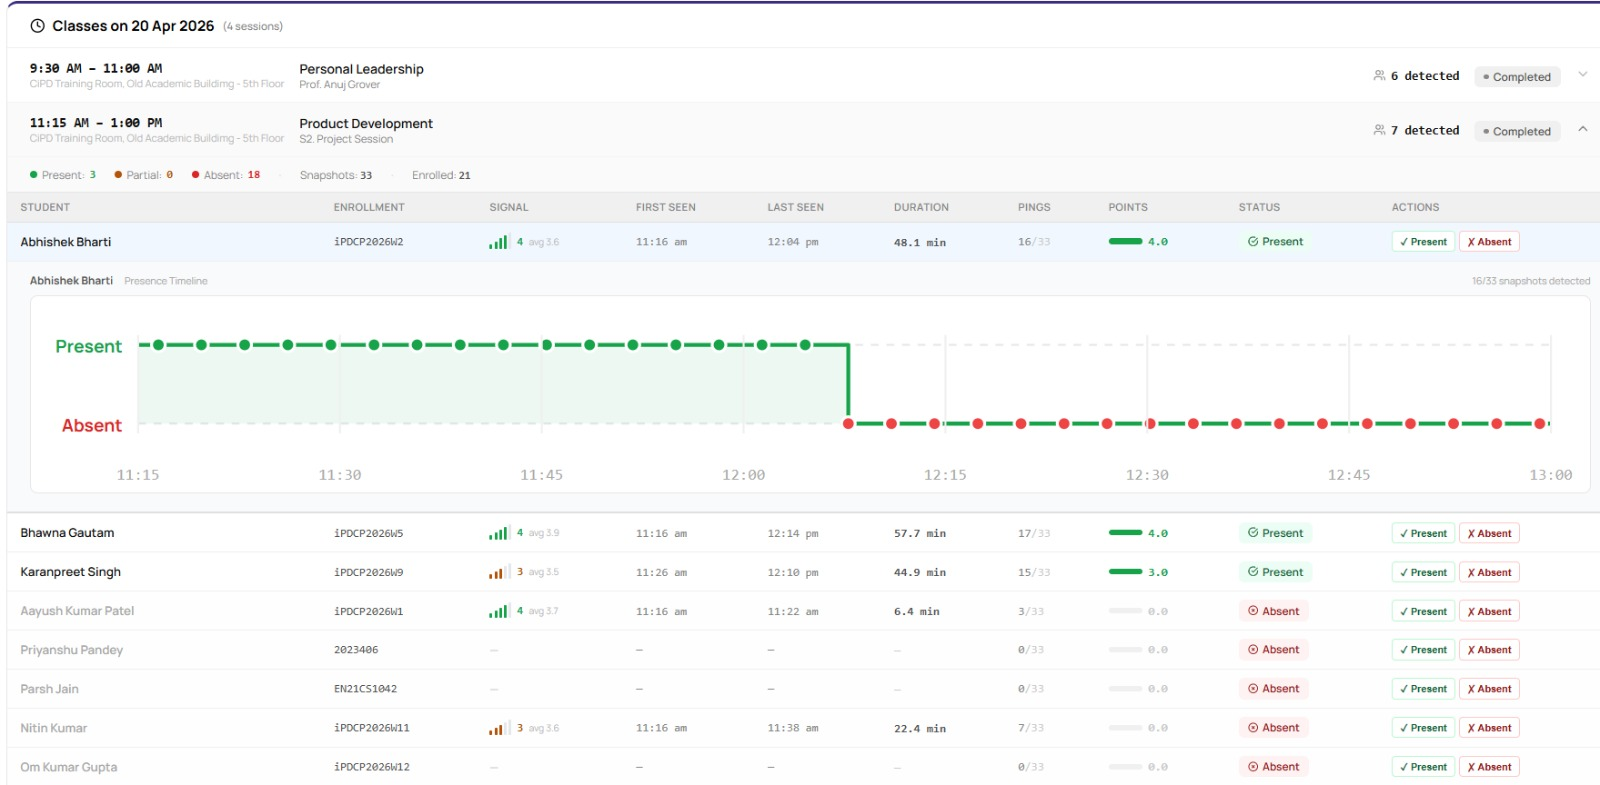
\includegraphics[width=0.95\textwidth]{images/4.jpeg}
    \caption{Session-level attendance detail showing per-student presence timeline, pings, signal strength, and computed points}
    \label{fig:session_detail}
\end{figure}

\subsection{Points Based Attendance Scoring}

To provide a more granular representation of participation, the system uses a points-based scoring
model instead of a simple present/absent classification.

Attendance is scored out of a total of 5 base points, with an additional bonus point awarded for
timely arrival.

\textbf{Scoring Logic:}

\begin{itemize}
    \item \textbf{Base Score (5 points):} Assigned based on overall presence during the session
    \item \textbf{Bonus Point (+1):} Awarded if the student's first detection occurs within 8 minutes of session
    start time
\end{itemize}

\textbf{Attendance Calculation (based on \% of detections):}

\begin{itemize}
    \item $\geq$ 85\% detections: Full attendance $\rightarrow$ 5 points
    \item 70\% $\leq$ detections $<$ 85\%: Slightly reduced $\rightarrow$ 4 points
    \item 50\% $\leq$ detections $<$ 70\%: Partial attendance $\rightarrow$ 3 points
    \item $<$ 50\% detections: Marked absent $\rightarrow$ 0 points
\end{itemize}

This model ensures that attendance scoring accounts for both duration of presence and punctuality,
providing a more accurate measure of student engagement. It also enables richer analytics compared
to a binary attendance system, supporting better evaluation of participation patterns.

% figs/scoring.tex — Attendance points scoring bar chart
\begin{figure}[!ht]
\centering
\begin{tikzpicture}
\begin{axis}[
  xbar, bar width=18pt,
  symbolic y coords={
    {Absent ($<$50\%)},
    {Partial (50--70\%)},
    {Reduced (70--85\%)},
    {Full ($\geq$85\%)}},
  ytick=data,
  xmin=0, xmax=6.5,
  xlabel={Points Awarded},
  title={Points-Based Attendance Scoring Model},
  nodes near coords, nodes near coords align={horizontal},
  every node near coord/.append style={font=\small},
  width=0.78\textwidth, height=5.5cm,
  xmajorgrids=true, grid style={dashed, gray!35},
  enlarge y limits=0.25,
]
\addplot[fill=accentblue!75, draw=accentblue] coordinates {
  (0,{Absent ($<$50\%)})
  (3,{Partial (50--70\%)})
  (4,{Reduced (70--85\%)})
  (5,{Full ($\geq$85\%)})
};
\end{axis}
\end{tikzpicture}
\caption{Points-based attendance scoring thresholds and corresponding values}
\label{fig:scoring}
\end{figure}


\subsection{Real Time Monitoring and Admin Controls}

The system provides a comprehensive interface for administrators to monitor attendance in real
time.

Key features include:

\begin{itemize}
    \item \textbf{Live Student Detection:} Displays currently detected devices during ongoing sessions
    \item \textbf{Session Level Analytics:} Shows number of detected students, total enrolled students, and
    session status. Can also view individual entry and exit time of students in each session.
    \item \textbf{Per Student Breakdown:} Detailed view including detection timestamps, signal strength,
    duration, and computed points
    \item \textbf{Manual Override:} Administrators can mark a student as present or absent in exceptional
    cases
    \item \textbf{Penalty Enforcement:} In cases of suspected misuse, penalties can be applied to discourage
    proxy attendance
\end{itemize}

These controls ensure that the system remains flexible and allows human intervention when
required.

\begin{figure}[!ht]
    \centering
    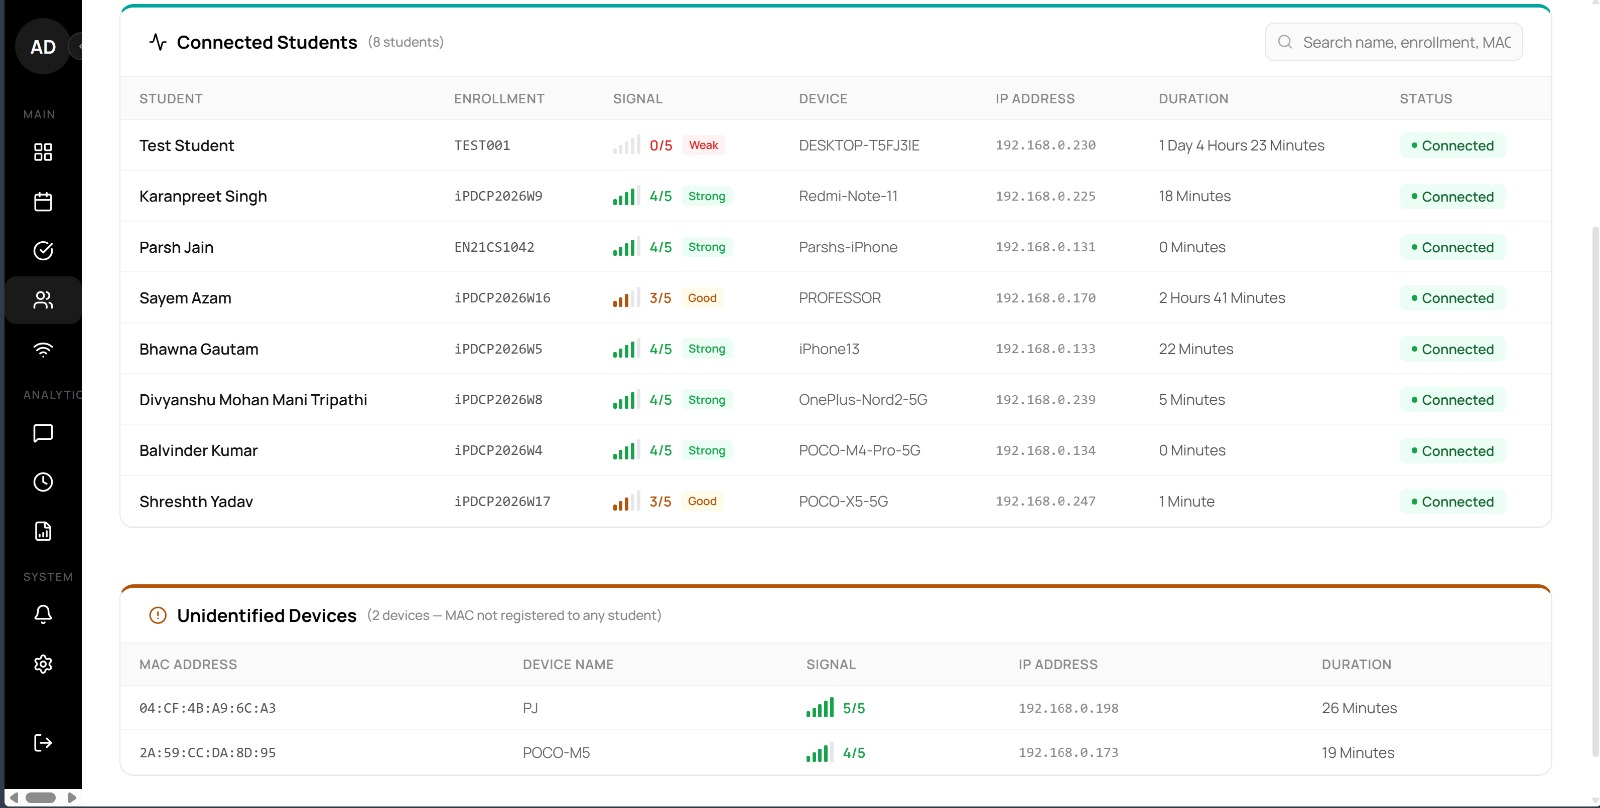
\includegraphics[width=0.95\textwidth]{images/1.jpeg}
    \caption{Real-time live detection view showing connected students with signal strength, device name, IP address, duration, and unidentified devices}
    \label{fig:live_detection}
\end{figure}

\subsection{Data Storage and Processing}

The attendance system maintains multiple layers of data for accuracy and auditability:

\begin{itemize}
    \item \textbf{Raw Data:} WiFi snapshots and ping logs containing detected devices
    \item \textbf{Processed Data:} Aggregated attendance records per student per session
    \item \textbf{Metadata:} Detection timestamps, signal strength, and duration of presence
\end{itemize}

Attendance records are updated dynamically and stored in a structured format, enabling both real
time access and historical analysis.

\subsection{Automation and Background Processing}

To ensure reliability, attendance processing is supported by automated background workflows.

\begin{itemize}
    \item Periodic processes analyze WiFi snapshots and compute attendance
    \item Sessions are automatically marked as completed after their scheduled duration
    \item Attendance records are finalized without requiring manual intervention
\end{itemize}

This reduces dependency on manual actions and ensures consistency in attendance data.

\subsection{Challenges and Limitations}

While the system provides significant advantages, it also introduces certain challenges:

\begin{itemize}
    \item Dependence on network availability and scanner reliability
    \item Potential inaccuracies due to weak signal strength or device disconnection
    \item Requirement for proper MAC registration and verification
\end{itemize}

\section{Feedback System}

The Feedback System is designed to capture structured student feedback for each lecture and
transform it into actionable insights for faculty and administrators. It serves as the qualitative
intelligence layer of the CIPD 360 ERP, using data to generate insights and actionable actions.

\subsection{Session Based Feedback Model}

The system follows a session driven feedback approach, where feedback forms are generated for
each completed session.

Key characteristics:

\begin{itemize}
    \item Feedback is linked directly to individual sessions
    \item Only eligible students (typically those associated with the session) can submit responses
    \item Feedback availability is time bound, with defined deadlines
\end{itemize}

This ensures that feedback is contextual, relevant, and collected shortly after the session, improving
response quality and accuracy.

\subsection{Feedback Collection Workflow}

The feedback process is tightly integrated with the session lifecycle:

\begin{enumerate}
    \item A session is marked as completed by the system or administrator
    \item The system triggers feedback availability for relevant students
    \item Students receive notifications regarding pending feedback
    \item Students access the feedback interface and submit responses
    \item Responses are stored and made available for analysis
\end{enumerate}

This workflow ensures minimal manual intervention and maintains consistency across all sessions.

\subsection{Feedback Form Structure}

The system supports multiple types of feedback questions to capture both quantitative and
qualitative responses.

Supported question formats include:

\begin{itemize}
    \item \textbf{Rating Scale (e.g., 1--5):} Used for evaluating aspects such as content quality, structure, and
    delivery
    \item \textbf{Yes/No Questions:} Used for binary assessments, such as whether a session started on time
    \item \textbf{Conditional Questions:} Follow up questions triggered based on previous responses
    \item \textbf{Descriptive/Text Responses:} Allow students to provide detailed feedback and suggestions
\end{itemize}

This flexible structure enables comprehensive evaluation of sessions while maintaining a simple user
experience.

\begin{figure}[!ht]
    \centering
    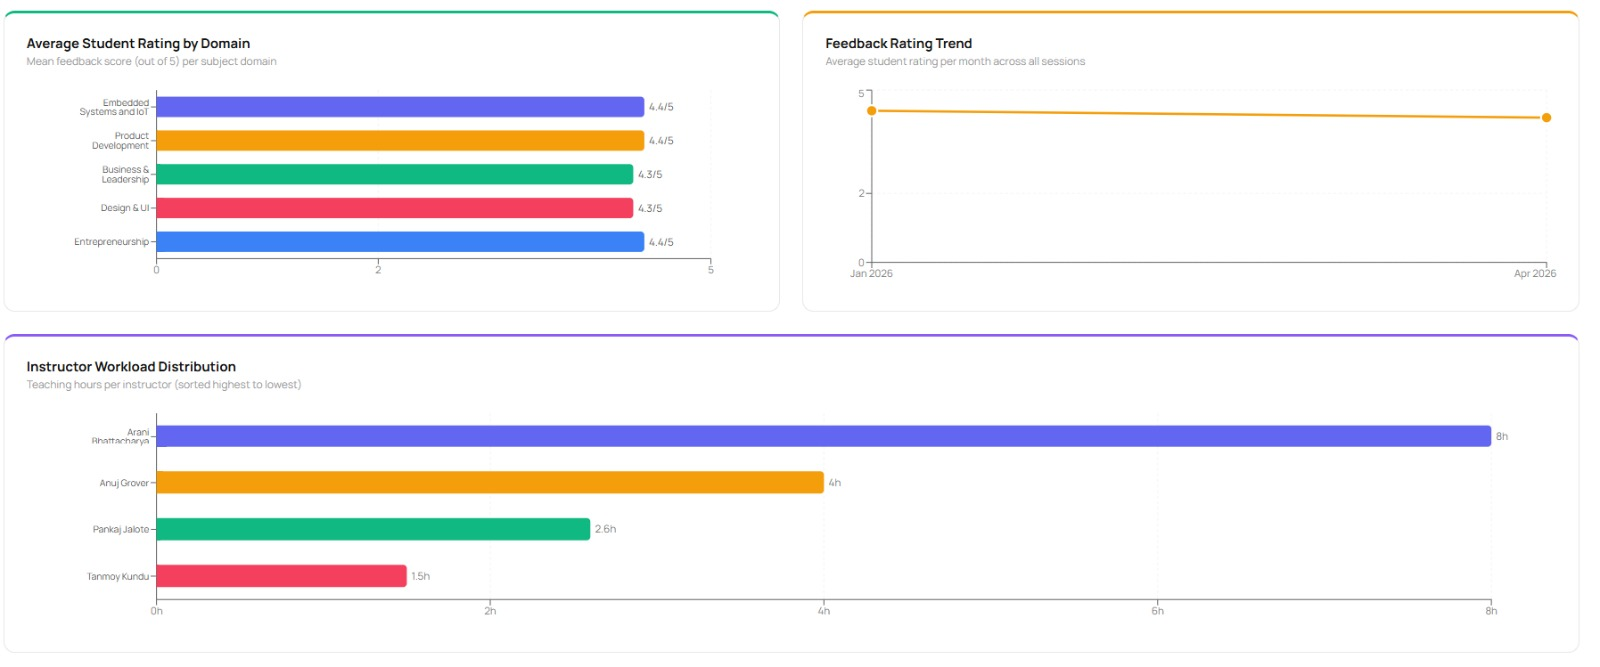
\includegraphics[width=0.90\textwidth]{images/6.jpeg}
    \caption{Student feedback submission interface for a completed session}
    \label{fig:feedback_form}
\end{figure}

\subsection{Feedback Submission Constraints}

To encourage higher participation rates, the system is designed for quick and efficient feedback
submission.

\begin{itemize}
    \item Feedback forms are optimized to be completed within a short duration (approximately one
    minute)
    \item Default selections or simplified input mechanisms are used to reduce friction
    \item Time bound availability ensures that feedback is submitted promptly
\end{itemize}

These design choices aim to balance usability with the need for meaningful data collection.

\subsection{Notification and Reminder System}

The system incorporates a notification driven approach to ensure timely feedback submission.

Key features include:

\begin{itemize}
    \item \textbf{Initial Notification:} Students are notified when feedback becomes available for a session
    \item \textbf{Reminder Notifications:} Students who have not submitted feedback receive reminders
    before the deadline
    \item \textbf{Administrative Control:} Administrators can trigger additional reminders if required
\end{itemize}

This approach improves submission rates and ensures that feedback data is sufficiently
comprehensive.

\subsection{Feedback Analytics and Insights}

Collected feedback is processed and presented through analytical dashboards for administrators and
faculty.

Key analytics include:

\begin{itemize}
    \item \textbf{Average Ratings:} Aggregated scores for different evaluation parameters
    \item \textbf{Response Distribution:} Breakdown of ratings across students
    \item \textbf{Submission Rates:} Percentage of students who submitted feedback for a session
    \item \textbf{Session Level Insights:} Comparative analysis across sessions, courses, or instructors
    \item \textbf{Descriptive Feedback Review:} Access to textual responses for qualitative insights
\end{itemize}

These analytics help identify patterns, strengths, and areas for improvement in teaching and session
management.

\begin{figure}[!ht]
    \centering
    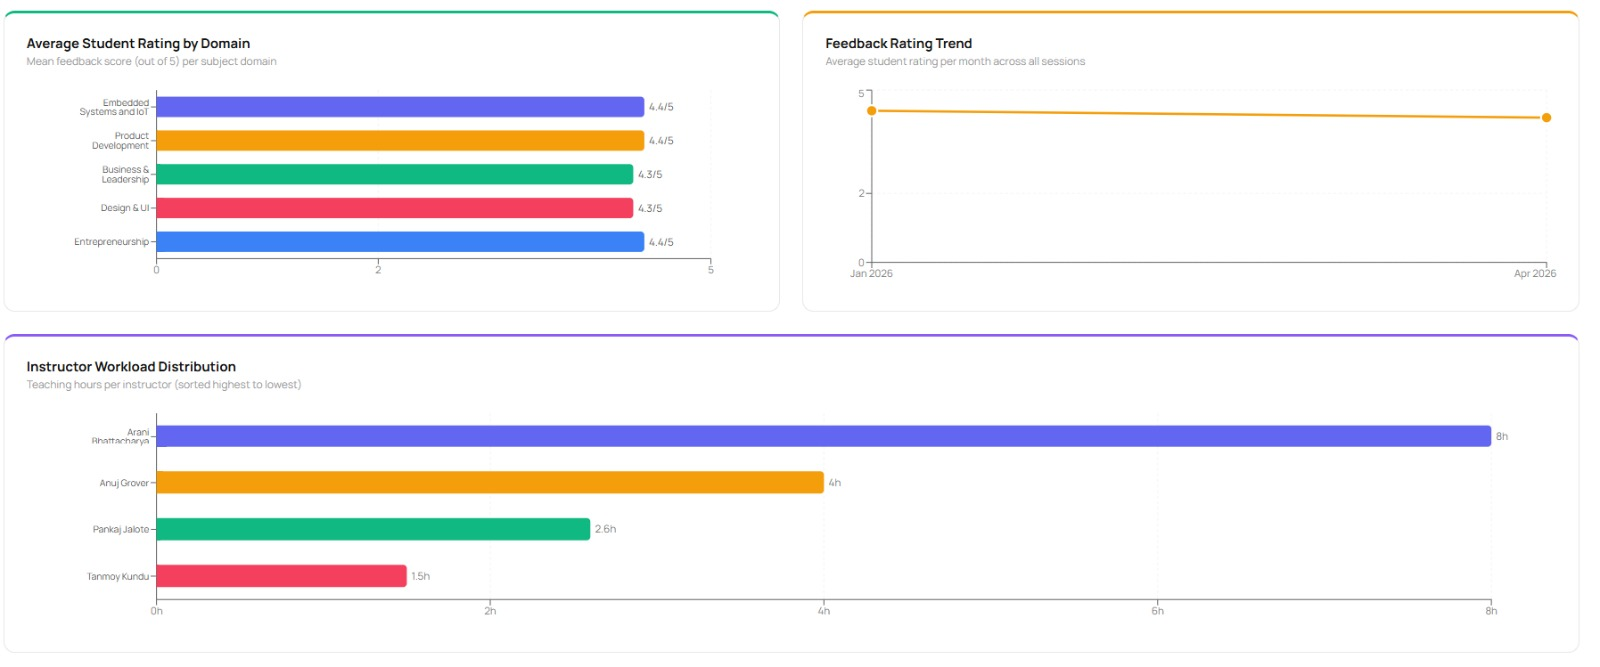
\includegraphics[width=0.95\textwidth]{images/6.jpeg}
    \caption{Feedback analytics dashboard showing average ratings by domain, feedback rating trend, and instructor workload distribution}
    \label{fig:feedback_analytics}
\end{figure}

\subsection{Design Considerations and Trade offs}

Several design decisions were made to balance usability and data quality:

\begin{itemize}
    \item \textbf{Notification Based Eligibility:} Feedback visibility is controlled through notifications, ensuring
    targeted distribution
    \item \textbf{Quick Submission Design:} Simplified forms increase participation but may reduce depth of
    responses
    \item \textbf{Time Bound Feedback Window:} Improves relevance but may lead to missed submissions if
    deadlines are too strict
    \item \textbf{Privacy Considerations:} Access to individual student responses is controlled to maintain
    confidentiality
\end{itemize}

These trade offs were carefully considered to ensure a practical and effective feedback system.

\section{Dashboard and Reporting}

The Dashboard and Reporting module provides a unified interface for visualizing system data and
deriving actionable insights. It serves as the presentation and analytics layer of the CIPD 360 ERP,
consolidating information from scheduling, attendance, and feedback into role specific views. This
enables users to monitor performance, track engagement, and make informed decisions.

\subsection{Role Based Dashboard Design}

The system implements dashboards tailored to different user roles:

\begin{itemize}
    \item \textbf{Administrator Dashboard:} Offers an overview of system activity, including attendance
    trends, session statistics, feedback summaries, and faculty workload, supporting monitoring
    and decision making.
    \item \textbf{Student Dashboard:} Displays personalized information such as upcoming sessions,
    attendance percentage, pending feedback, learning resources, and assignments.
\end{itemize}

Dashboards are dynamically populated based on user roles, ensuring relevance and clarity.

\begin{figure}[!ht]
    \centering
    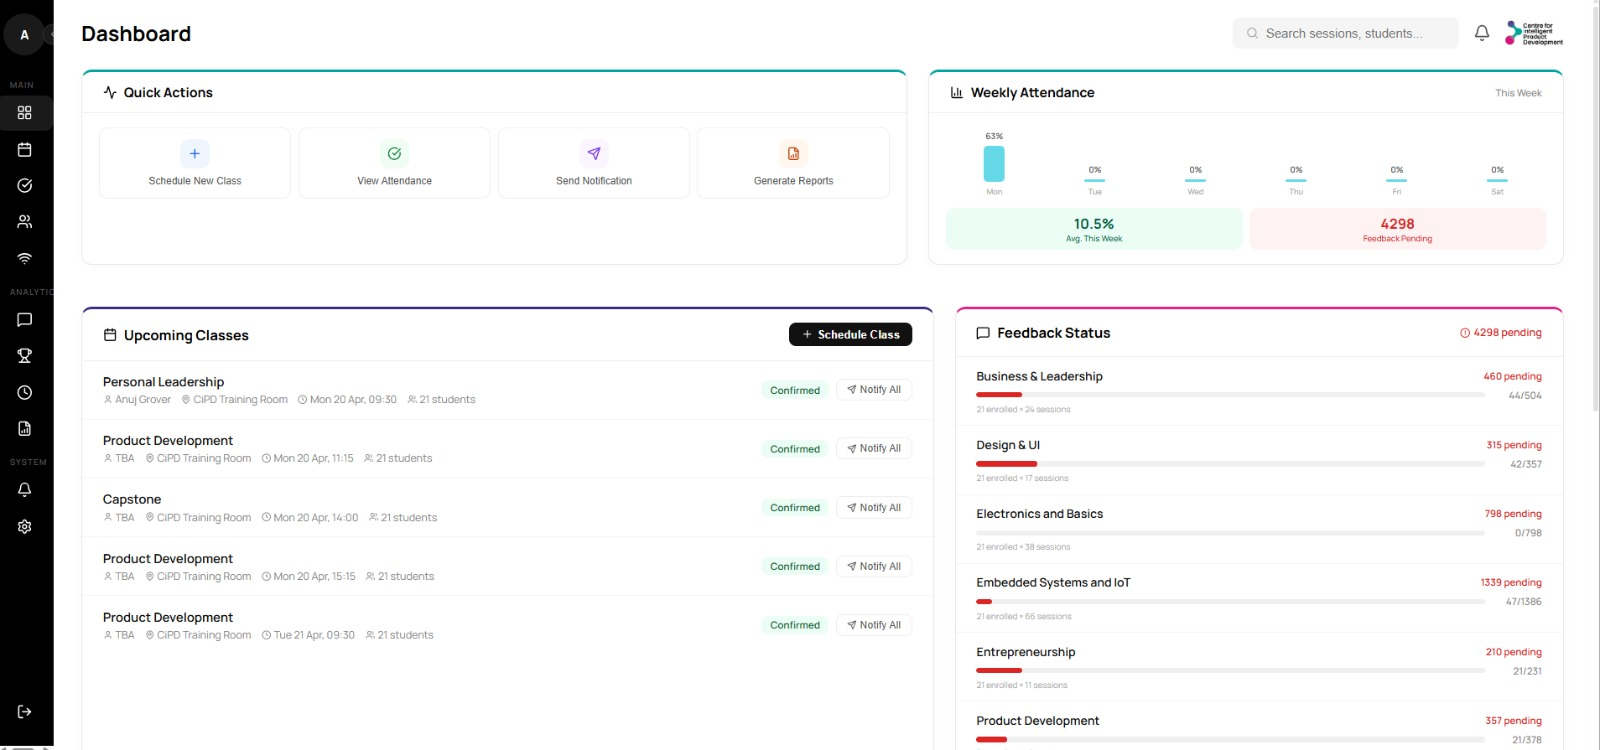
\includegraphics[width=0.95\textwidth]{images/7.jpeg}
    \caption{Admin dashboard showing quick actions, weekly attendance chart, upcoming classes list, and per-course feedback status}
    \label{fig:admin_dashboard}
\end{figure}

\begin{figure}[!ht]
    \centering
    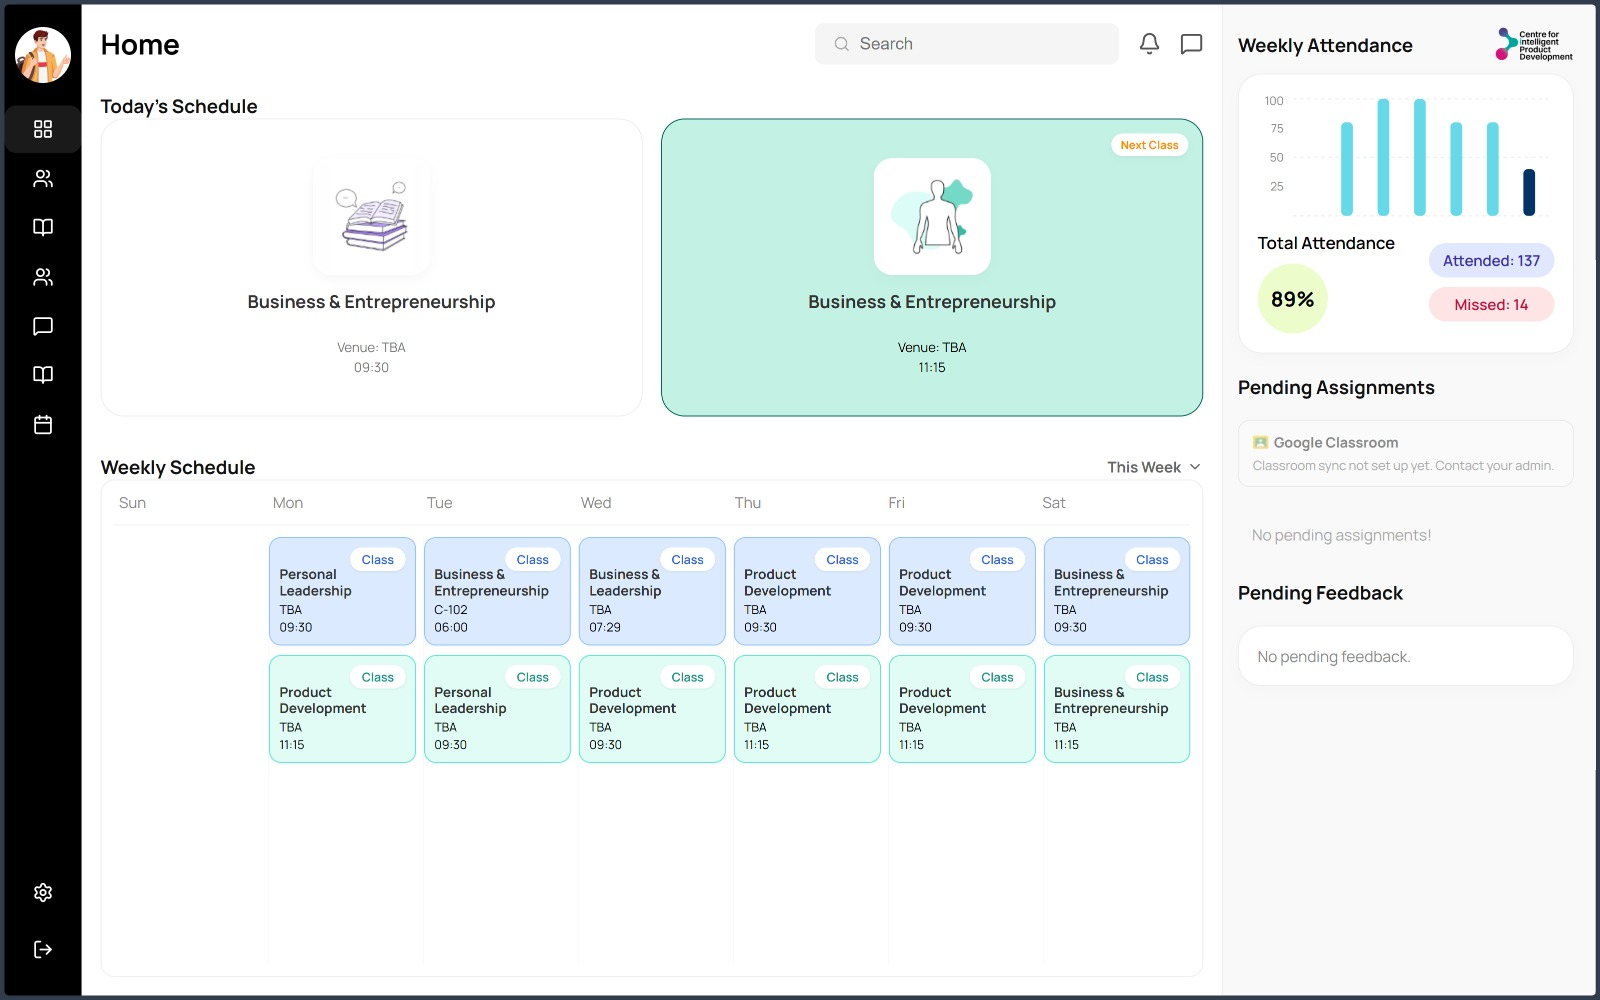
\includegraphics[width=0.95\textwidth]{images/2.jpeg}
    \caption{Student home dashboard showing today's schedule, weekly calendar view, total attendance (89\%), pending assignments, and pending feedback}
    \label{fig:student_dashboard}
\end{figure}

\subsection{Key Dashboard Components}

Dashboards consist of components that provide both summary and detailed insights:

\begin{itemize}
    \item \textbf{Cards:} Display key metrics such as attendance percentage, session counts, and pending tasks
    \item \textbf{Graphs and Visualizations:} Show trends in attendance, feedback, and participation
    \item \textbf{Activity Panels and Alerts:} Highlight recent updates and notify users of pending actions
\end{itemize}

These elements provide a balance between overview and actionable information.

\subsection{Analytics and Insights}

The reporting system generates insights across multiple dimensions:

\begin{itemize}
    \item \textbf{Attendance Analytics:} Includes time based trends, course wise analysis, and student level
    participation metrics
    \item \textbf{Feedback Analytics:} Covers average ratings, response distributions, submission rates, and
    qualitative responses
    \item \textbf{Faculty and Session Analytics:} Tracks sessions conducted, teaching hours, and engagement
    levels
\end{itemize}

These analytics help identify patterns, evaluate performance, and support decision making.

\begin{figure}[!ht]
    \centering
    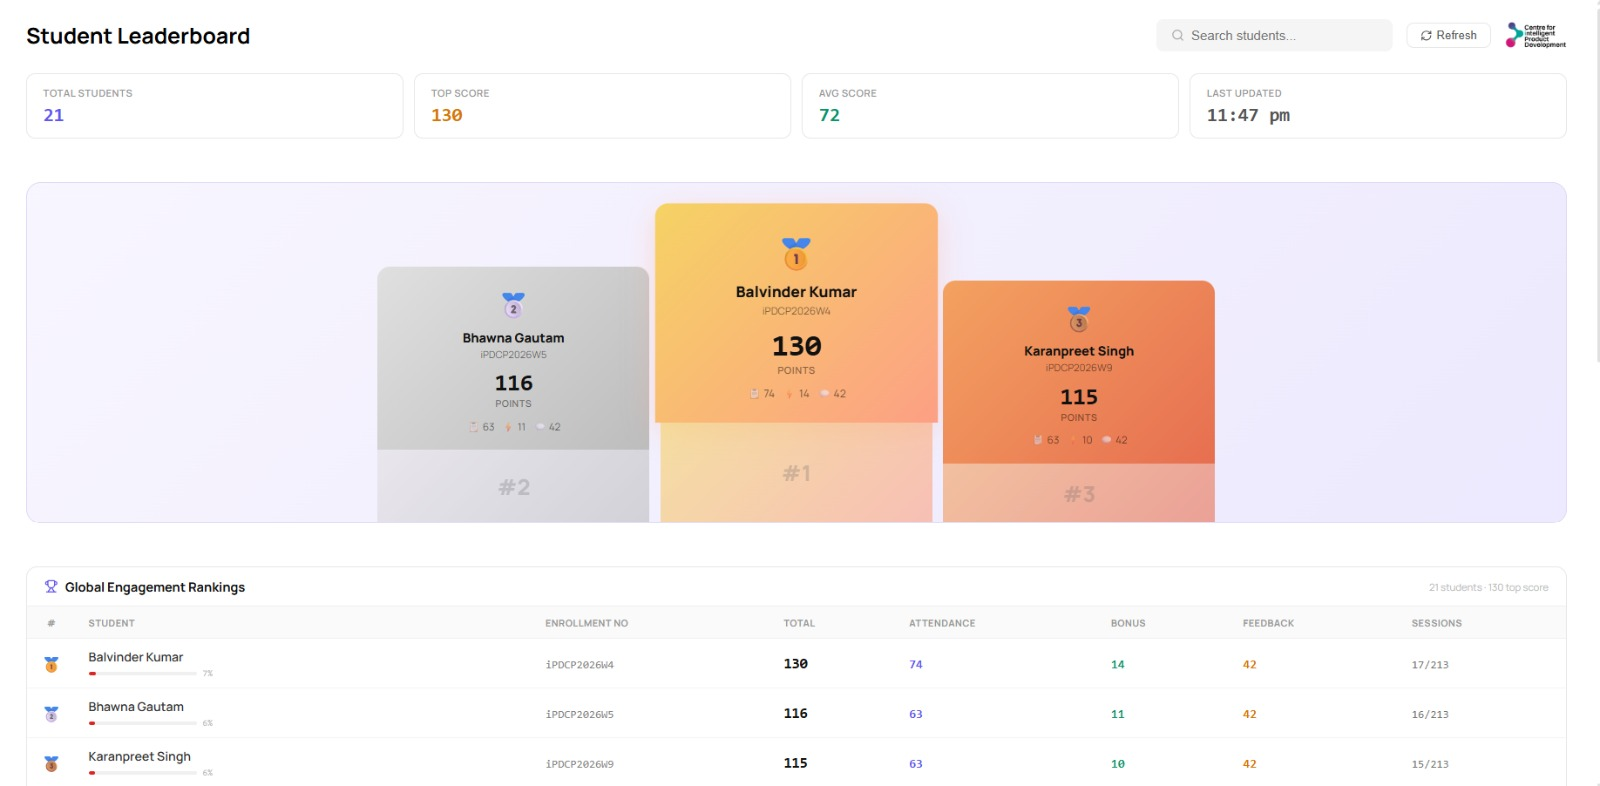
\includegraphics[width=0.95\textwidth]{images/5.jpeg}
    \caption{Student engagement leaderboard showing global rankings by total points, attendance score, bonus points, feedback score, and sessions attended}
    \label{fig:leaderboard}
\end{figure}

\subsection{Reporting and Data Export}

The system supports generation of structured reports for administrative use:

\begin{itemize}
    \item Report types include attendance, feedback, and session analytics
    \item Export options such as CSV and PDF are supported
    \item Filters allow customization based on date, course, or user group
\end{itemize}

This functionality enables efficient data sharing and external analysis.

\section{Content and Assignment System}

\subsection{Course Centric Content Management}

The system organizes academic content in a course-centric manner, where materials are associated
with specific sessions and courses. A total of 10 modules/courses have been implemented:

\begin{multicols}{2}
\begin{itemize}
    \item Business \& Entrepreneurship
    \item Entrepreneurship
    \item Business \& Leadership
    \item Personal Leadership
    \item Electronics and Basics
    \item Capstone
    \item Embedded Systems and IoT
    \item Product Development
    \item Software \& App Development
    \item Design \& UI
\end{itemize}
\end{multicols}

Key features include:

\begin{itemize}
    \item \textbf{Lecture Material Upload:} Faculty and administrators can upload resources such as slides,
    PDFs, reference links, and notes
    \item \textbf{Session-Based Association:} Materials are linked to specific sessions for contextual access
    \item \textbf{Centralized Access:} Students can access all materials through a unified interface
\end{itemize}

Additionally, the system incorporates a structured skills framework with 100+ engineering and
product development skills across 46 categories, enabling better alignment of coursework with
learning outcomes.

\begin{figure}[!ht]
    \centering
    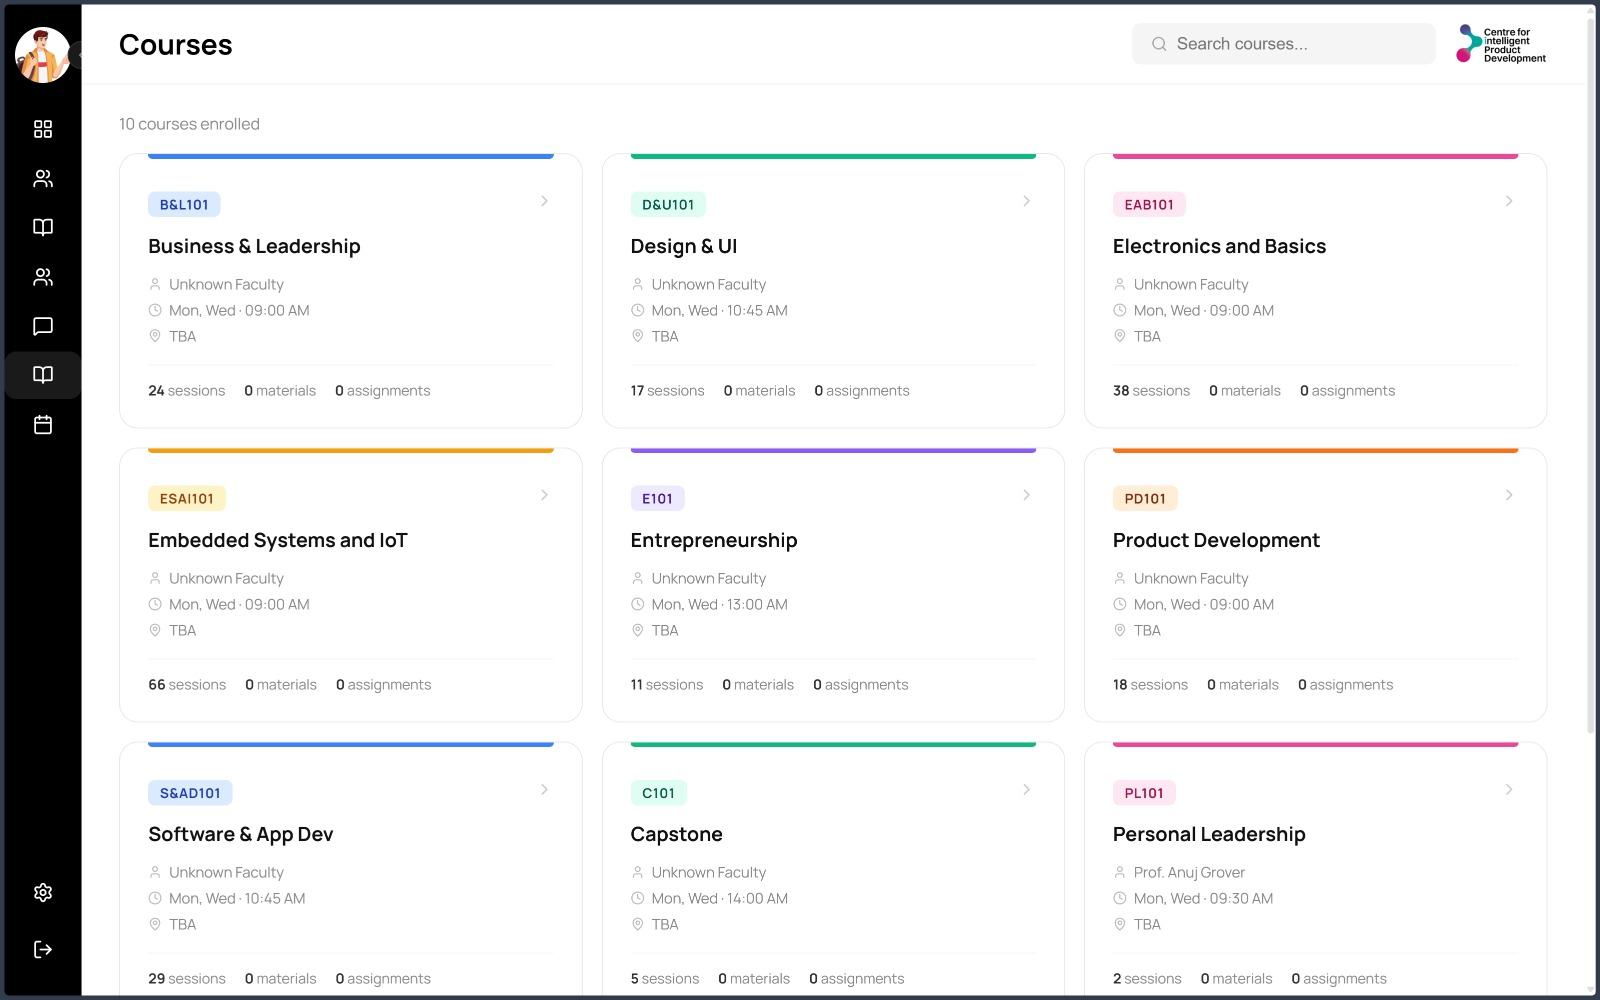
\includegraphics[width=0.95\textwidth]{images/3.jpeg}
    \caption{Student courses page showing all 10 enrolled modules with session counts, materials, and assignments}
    \label{fig:courses_page}
\end{figure}

\subsection{Role Based Content Access}

Access to content is governed by user roles:

\begin{itemize}
    \item \textbf{Faculty/Admin:} Can upload, update, and manage content and assignments
    \item \textbf{Students:} Can view and download materials
\end{itemize}

This ensures content integrity while maintaining ease of use.

\subsection{Assignment Management and Submissions}

The system provides a structured workflow for assignment management:

\begin{itemize}
    \item \textbf{Assignment Creation:} Faculty can define assignments with title, description, and deadlines
    \item \textbf{Course/Session Mapping:} Assignments are linked to relevant courses or sessions
    \item \textbf{Student Access:} Assignments are accessible via dashboards and course pages
\end{itemize}

For submissions:

\begin{itemize}
    \item \textbf{File Upload Support:} Students can submit documents such as PDFs or reports
    \item \textbf{Submission Metadata:} The system records timestamps, student identity, and version details
    \item \textbf{Version Handling:} Multiple submissions are supported before deadlines
\end{itemize}

Faculty can evaluate submissions by assigning marks and providing feedback, which is visible to
students.

\subsection{Integration with Google Classroom}

The system integrates with Google Classroom using OAuth-based authentication.

\begin{itemize}
    \item Assignments created in Google Classroom are automatically fetched and displayed within
    the ERP
    \item Students can view both ERP and Google Classroom assignments in a single dashboard
    \item Eliminates the need to switch platforms while ensuring consistency
\end{itemize}

This integration extends functionality without duplicating existing systems and improves overall
usability.

\subsection{Dashboard Integration}

The module is integrated with the dashboard to enhance visibility:

\begin{itemize}
    \item Students can track pending assignments and upcoming deadlines
    \item Faculty can monitor submission status and progress
\end{itemize}

This ensures users remain informed and improves task management efficiency.

\subsection{Role in Overall System}

The Content and Assignment System supports:

\begin{itemize}
    \item Delivery of learning resources
    \item Management of coursework
    \item Tracking of academic performance
\end{itemize}

By integrating with scheduling, attendance, and feedback modules, it contributes to a cohesive and
comprehensive academic management system.
